% !TEX TS-program = xelatex
\documentclass[a4paper, 10pt]{article}
\usepackage{a4wide}
%\usepackage[T1]{fontenc}
\usepackage[utf8]{inputenc}
\usepackage[spanish]{babel}
\usepackage[none]{hyphenat}
\usepackage{xltxtra,fontspec,xunicode}
\setromanfont[Numbers=Uppercase]{Helvetica Light}
\usepackage{hyperref}
\usepackage[top=40pt,bottom=50pt,left=48pt,right=46pt]{geometry}
\usepackage{tabularx}
\usepackage{enumitem}
\usepackage{titling}
\usepackage{multicol}
\usepackage{graphicx}
\usepackage{color}
\usepackage{xcolor}
\usepackage{framed}
\usepackage{tikz}
\usepackage{scrextend}
\usepackage{wrapfig}
\usepackage{float}
\usepackage{calc}


\usetikzlibrary{decorations.pathreplacing}
\usetikzlibrary{shadows}
\usetikzlibrary{calc}

		\definecolor{darkgray}{HTML}{3C3C3C}
		\definecolor{lightgray}{HTML}{6C6C6C}


		\newcommand{\CVSection}[1]{ {\setromanfont[Numbers=Uppercase]{Helvetica}\selectfont \section*{#1}} }
		\newcommand{\CVSubsection}[1]{ { \setromanfont[Numbers=Uppercase]{Helvetica}\selectfont \subsection*{#1} } }
		\newcommand{\CVComment}[1]{{\fontsize{0.75em}{1em}\selectfont #1}}

		%\titleformat{\section}{\large\bfseries\setromanfont[Numbers=Uppercase]{Corbel}\selectfont}{}{0pt}{\thesection}

		\renewenvironment{leftbar}[1][\hsize]
		{%
		    \def\FrameCommand
		    {%
		        {\color{darkgray}\vrule width 2pt}%
		        %\hspace{0pt}%must no space.
		        %\fboxsep=\FrameSep\colorbox{yellow}%
		    }%
		    \MakeFramed{\hsize#1\advance\hsize-\width\FrameRestore}%
		}
		{\endMakeFramed}

		\makeatletter
		\newcommand{\gettikzxy}[3]{%
		  \tikz@scan@one@point\pgfutil@firstofone#1\relax
		  \edef#2{\the\pgf@x}%
		  \edef#3{\the\pgf@y}%
		}
		\makeatother

		\newenvironment{timeline}{
			\begin{leftbar}
		}{
			\end{leftbar}
		}

		\setlength\parindent{0pt}

		\newenvironment{job}[1][date]{
			\newcommand{\jobdate}{#1}

			\begin{flushright}
			\begin{minipage}{0.88\linewidth}
			\tikz[remember picture] \node[coordinate,yshift=0.5em] (start) {};
		}{
			\tikz[remember picture] \node[coordinate] (end) {};
			%\xdef\tpd{\the\prevdepth}
			\end{minipage}
			\end{flushright}

			\begin{tikzpicture}[overlay,remember picture]

				\pgfmathsetmacro\triangleLength{0.4}
				\pgfmathsetmacro\halfTriangleLength{(\triangleLength/2)}

				\gettikzxy{(start)}{\startx}{\starty}
				\gettikzxy{(end)}{\endx}{\endy}

				\node[coordinate] (start) at (\startx-10pt,\starty) {};
				\node[coordinate] (end) at (\startx-10pt,\endy-5pt) {};

				\node[coordinate] (middle) at ($(start)!0.5!(end)$) {};

				\node[coordinate] (triangle-up) at ($(middle) + (0, \halfTriangleLength)$) {};
				\node[coordinate] (triangle-down) at ($(middle) + (0, -\halfTriangleLength)$) {};
				\node[coordinate] (triangle-tip) at ($(middle) + (-\halfTriangleLength, 0)$) {};

				\draw[thick, lightgray]
					(start) -- (triangle-up) -- (triangle-tip) -- (triangle-down) -- (end);

				\node (date) at (triangle-tip) [left, text width=1.3cm, align=center] {\jobdate};

				%\foreach \xy in {start, triangle-up, triangle-down, end}{
		 		%   \node at (\xy) {\xy};
				%}

		  	\end{tikzpicture}
		}





		\def\shadowshift{3.5pt,-3.5pt}
		\def\shadowradius{2pt}

		\colorlet{innercolor}{gray!30}
		\colorlet{outercolor}{gray!01}

		% this draws a shadow under a rectangle node
		\newcommand\drawshadow[1]{
		    \begin{pgfonlayer}{shadow}
		        \shade[outercolor,inner color=innercolor,outer color=outercolor] ($(#1.south west)+(\shadowshift)+(\shadowradius/2,\shadowradius/2)$) circle (\shadowradius);
		        \shade[outercolor,inner color=innercolor,outer color=outercolor] ($(#1.north west)+(\shadowshift)+(\shadowradius/2,-\shadowradius/2)$) circle (\shadowradius);
		        \shade[outercolor,inner color=innercolor,outer color=outercolor] ($(#1.south east)+(\shadowshift)+(-\shadowradius/2,\shadowradius/2)$) circle (\shadowradius);
		        \shade[outercolor,inner color=innercolor,outer color=outercolor] ($(#1.north east)+(\shadowshift)+(-\shadowradius/2,-\shadowradius/2)$) circle (\shadowradius);
		        \shade[top color=innercolor,bottom color=outercolor] ($(#1.south west)+(\shadowshift)+(\shadowradius/2,-\shadowradius/2)$) rectangle ($(#1.south east)+(\shadowshift)+(-\shadowradius/2,\shadowradius/2)$);
		        \shade[left color=innercolor,right color=outercolor] ($(#1.south east)+(\shadowshift)+(-\shadowradius/2,\shadowradius/2)$) rectangle ($(#1.north east)+(\shadowshift)+(\shadowradius/2,-\shadowradius/2)$);
		        \shade[bottom color=innercolor,top color=outercolor] ($(#1.north west)+(\shadowshift)+(\shadowradius/2,-\shadowradius/2)$) rectangle ($(#1.north east)+(\shadowshift)+(-\shadowradius/2,\shadowradius/2)$);
		        \shade[outercolor,right color=innercolor,left color=outercolor] ($(#1.south west)+(\shadowshift)+(-\shadowradius/2,\shadowradius/2)$) rectangle ($(#1.north west)+(\shadowshift)+(\shadowradius/2,-\shadowradius/2)$);
		        \filldraw[color=innercolor] ($(#1.south west)+(\shadowshift)+(\shadowradius/2,\shadowradius/2)$) rectangle ($(#1.north east)+(\shadowshift)-(\shadowradius/2,\shadowradius/2)$);
		    \end{pgfonlayer}
		}

		% create a shadow layer, so that we don't need to worry about overdrawing other things
		\pgfdeclarelayer{shadow} 
		\pgfsetlayers{shadow,main}


		\newcommand\shadowimage[2][]{%
		\begin{tikzpicture}
		\node[anchor=south west,inner sep=0] (image) at (0,0) {\includegraphics[#1]{#2}};
		\drawshadow{image}
		\end{tikzpicture}}



		\pagenumbering{gobble}


		\newcommand{\onlineCourse}[3]{
			\begin{minipage}{\linewidth}
				\begin{wrapfigure}{L}{0.15\linewidth} 
					\vspace{#3}
					\includegraphics[width=\linewidth]{#1}
				\end{wrapfigure} {\vspace{4mm}#2\vspace{3mm}}
			\end{minipage}
		}

		\newcommand{\skill}[5]{
			\begin{minipage}{0.85\linewidth}
				\begin{wrapfigure}{L}{0.15\linewidth} 
					\vspace{#3}

					\hspace*{#5}\includegraphics[width=#4]{#1}
				\end{wrapfigure} {#2}
			\end{minipage}
		}


\begin{document}

	\null

	\vspace{0.3cm}

	% PICTURE
	\begin{minipage}{0.23\linewidth}   

		\vspace{70pt}
		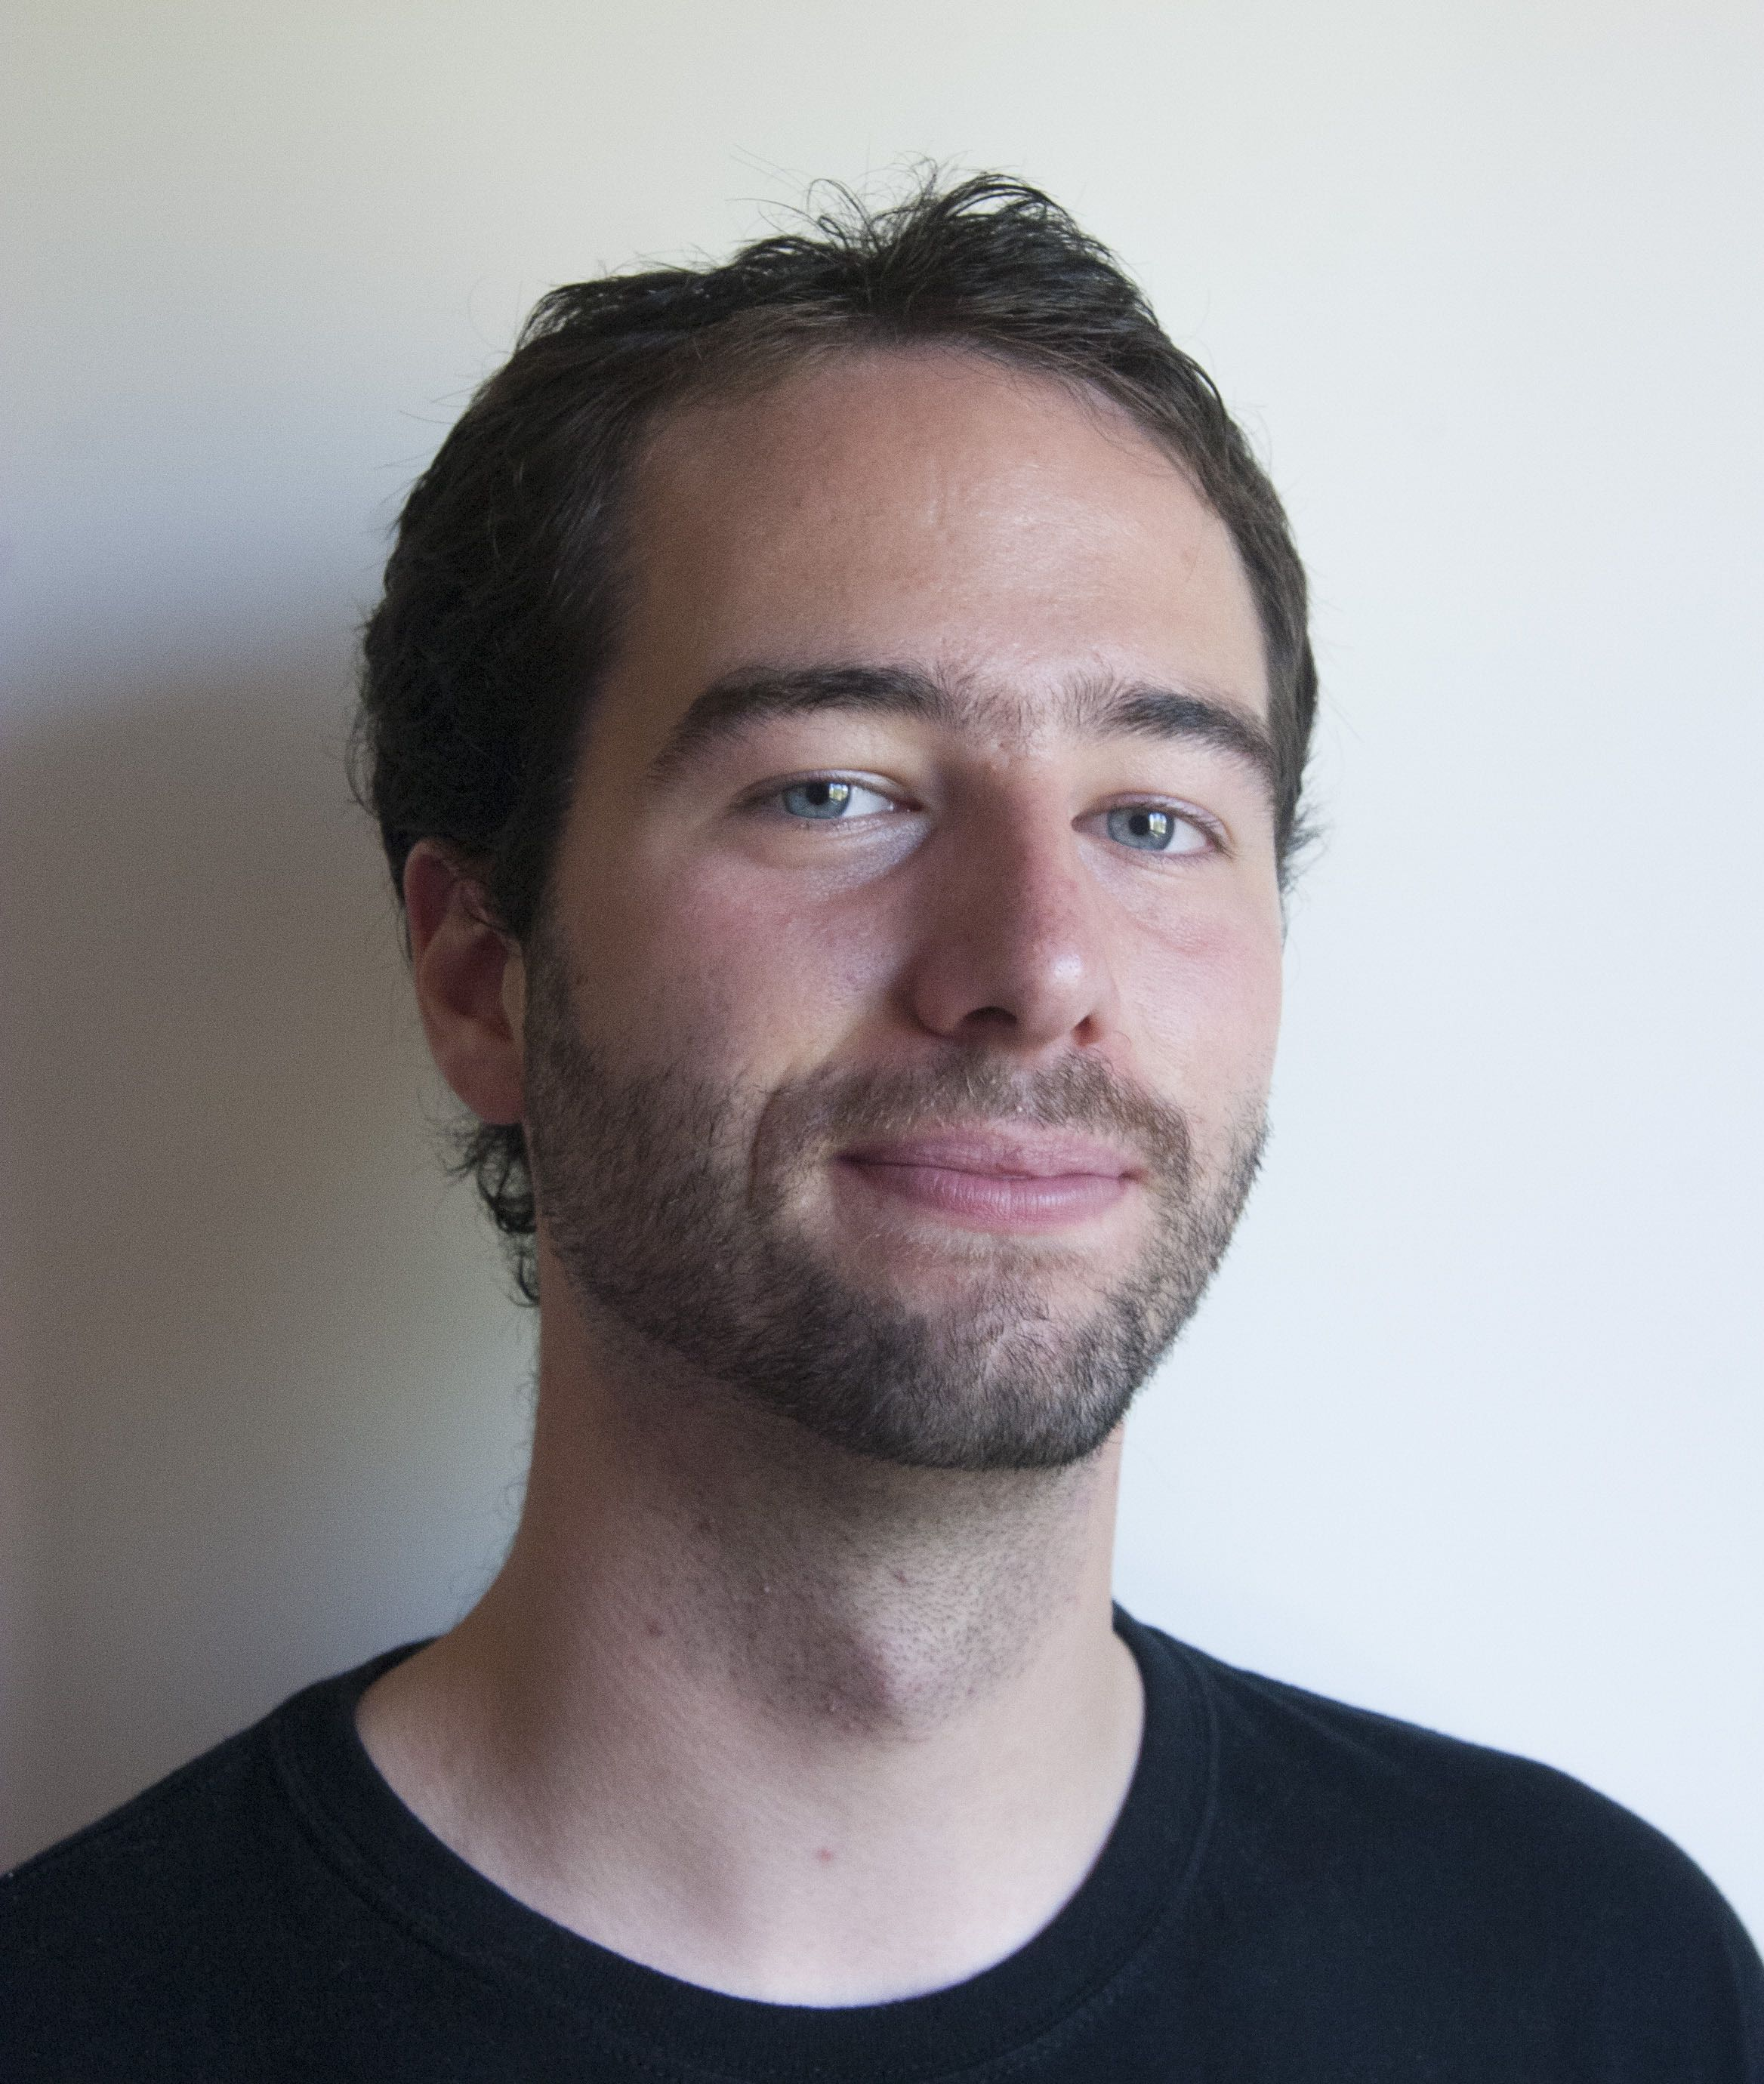
\includegraphics[width=0.20\linewidth]{images/me.jpg}

	\end{minipage}% TITLE and SUBTITLES
	\begin{minipage}{0.75\linewidth}

		\begin{flushright}

			\vspace{-25pt}

	  	{\setromanfont[Numbers=Uppercase]{Corbel}\selectfont {\fontsize{4em}{1em}\selectfont Guillermo Guridi}}

	  	\vspace{25pt}

		{\setromanfont[Numbers=Uppercase]{Helvetica Light}\selectfont

			{\fontsize{1.6em}{2em}\selectfont Computer Engineering and Mathematics student

			Web app developer (frontend and backend)

			}
		}

	\end{flushright}

	\end{minipage}

	\vspace{0.5cm}



	\begin{multicols}{2}
	  \begin{minipage}{0.9\linewidth}

		\begin{center}
		\CVSection{Experience}
		\end{center}

			\vspace{-2mm}

			\CVSubsection{Freelance Developer}
				\vspace{-2.5mm}
				\textit{\textbf{2010 - now} : Mediafire, Deexme, Qandell, oDesk...}

				\vspace{1mm}
				I've worked for 5 years as a freelance developer, developing full websites (design, backend and frontend) and iOS apps for different clients. Last year I did it through oDesk and got hired by Mediafire for three months.

				\vspace{1mm}
				I think I have gained plenty of experience treating with technical and not technical clients as well as planing and estimating development costs.



			\vspace{4.5mm}
			\CVSubsection{Research intern in sidechannel attacks}
				\vspace{-2.5mm}
				\textit{\textbf{summer 2013} : IMDEA Software Institute (Madrid)}

				\vspace{1mm}
				I helped program a static assembly analyzer that would derive leackage upper bounds for different cache-related sidechannel attacks. Also run some experiments with popular encription algorithms.




			\vspace{4.5mm}
			\CVSubsection{Small open-source projects}
				\vspace{-2.5mm}
				\textit{Two projects of my own and small contributions}

				\vspace{1mm}
				I've worked in many many projects on my own, just for fun or to keep learning, and I've published the ones I've considered worth it. An angularjs library for reactive save, refresh, etc... buttons and a 'blogging' platform I built for myself.

				\vspace{1mm}
				I've also contributed to some open source projects. Mostly when I've had to use them and found something broken or missing.



			\vspace{4.5mm}
			\CVSubsection{Participation in several Hackathons}
				\vspace{-2.5mm}
				\textit{Spotify WOWHack, GBG Startup hack, HackMed...}

				\vspace{1mm}
				I love hackathons and I haven't missed the chance to attend a lot of them. Most of the times I have built websites, but I have even built a RaspberryPi project once, and a small videogame another. And I'm proud to say I have won 3 times.


	  \end{minipage}

	  \vfill
	  \null


	  \columnbreak

		\begin{center}
		\CVSection{Knowledge}
		\end{center}

			\vspace{-10mm}

			Apart from the knowledge I've adquired at university I've complimented my studies with small jobs and personal projects to further increase my CS knowledge.

			\vspace{-5mm}

			\CVSubsection{Studies}
				\vspace{-3mm}
				I'm currently close to finishing my double bachelor in \textbf{Mathematics and Computer Engineering} at Universidad Autonoma de Madrid.

				\vspace{1mm}

				I studied one year in Sweden with the \textbf{Erasmus} programme.

				\vspace{1mm}

				I've had an \textbf{Academic Excellence Grant} and I have completed 10 courses with \textbf{special distinction}.


			\vspace{2mm}
			\CVSubsection{Skills}

				\vspace{-2mm}

				\setlength{\leftskip}{1.3cm}

				\skill{images/html5.png}{I have experience building complex and complete websites, both frontend (jquery, angularjs or vanilla) and backend (php, ruby on rails, nodejs).}{-3mm}{1.2cm}{0.5mm}

				\vspace{2mm}

				\skill{images/linux.png}{I'm familiar with GNU Linux environments, both as user and admin level. I've deployed servers on Amazon AWS using among others Apache, MySQL, Ruby on Rails, Glassfish, CouchDB, Docker...}{-4mm}{1.2cm}{0.5mm}

				\vspace{2mm}

				\skill{images/raspberry.png}{I've worked with embeded systems such as RaspberryPi or Arduino.}{-4.5mm}{0.8cm}{2.2mm}

				\vspace{2mm}

				\skill{images/tex.png}{I have quite some knowledge of LaTeX and I use it for most of my projects. Like this one.}{-6mm}{0.9cm}{2.2mm}

				\vspace{2mm}

				\skill{images/photoshop.png}{I am proficient in the use of graphic design tools such as Adobe Photoshop.}{-5mm}{0.8cm}{2.5mm}

				\vspace{2mm}

				\skill{images/git.png}{I use git to manage almost everything I do. My github profile is http://github.com/erpheus}{-4.5mm}{0.8cm}{2.5mm}	

				\setlength{\leftskip}{0mm}

				\vspace{2mm}
				\CVSubsection{Languages}
				\vspace{-2mm}
				{\fontsize{1.1em}{1em}\selectfont \textbf{Spanish}} is my mother tongue, I have fully proficient {\fontsize{1.1em}{1em}\selectfont \textbf{English}} level both written and spoken, and I am a beginner in {\fontsize{1.1em}{1em}\selectfont \textbf{French}} and {\fontsize{1.1em}{1em}\selectfont \textbf{Swedish}} although I would like to learn more.		


	\end{multicols}

	\vfill

	{\fontsize{1.35em}{1.4em}\selectfont 
		I’m a really passionate person regarding work. I enjoy solving computer science and mathematical problems and I love challenges. This passion keeps me constantly learning new things. I can get up to a reasonable ammount of fluency with new technologies quite quickly.

		\vspace{2mm}

		I don’t mind working individually but I would rather work inside a team, even if remotely.
	}

	\vfill

	\vfill

	\begin{minipage}{0.33\textwidth}
		\begin{center}
			http://github.com/erpheus
		\end{center}
	\end{minipage}
	\begin{minipage}{0.33\textwidth}
		\begin{center}
			http://about.me/erpheus
		\end{center}
	\end{minipage}
	\begin{minipage}{0.33\textwidth}
		\begin{center}
			guillermo@guridi.com
		\end{center}
	\end{minipage}



	\pagebreak

	\begin{center}
	\CVSection{Additional knowledge}
	\end{center}

		\vspace{1mm}

		\begin{multicols}{2}

			\CVSubsection{Completed online courses}

				\vspace{-4mm}
				\CVComment{in Coursera, Udacity y others.}

				\setlength{\leftskip}{1.6cm}

				\onlineCourse{images/ML.png}{Machine Learning (2011)}{-8mm}

				\onlineCourse{images/DB.png}{Introduction to databases (2011)}{-8mm}

				\onlineCourse{images/AI.png}{Introduction to AI (2011) \\ and AI for robotics (2012)}{-7mm}

				\onlineCourse{images/SAAS.png}{Sw. engineering for SaaS (2012)}{-8mm}

				\onlineCourse{images/CRIPTO.png}{Criptography (2012)}{-10mm}

				\onlineCourse{images/CISCO.png}{Cisco Network Fundamentals (2013)}{-8mm}


				\setlength{\leftskip}{0pt}

				\vfill
				\null


			\columnbreak

			\CVSubsection{Technologies I'm already confortable with}

				\vspace{-4mm}
				\CVComment{and some frameworks}

				\vspace{3mm}

				
\includegraphics[width=0.9\linewidth]{images/languages.png}


				\vfill
				\null


		\end{multicols}


		\CVSubsection{Extra curricular activities}

			\vspace{-2mm}
			I have a deep interest in photography and music. I'm an amateur photographer and musician (I can play piano and guitar).

			I also love cycling, hiking and travelling in general.


	\vspace{9mm}


	\begin{center}
	\CVSection{Open Source Projects}
	\end{center}

	\vspace{-1.3cm}

		\begin{timeline}

			\begin{job}[4/2015]

				\textbf{angular-promise-react}

				Available in github and bower. It is an angular library that helps making buttons that correspond to long lasting actions and show updates on those actions as well as the output on the button itself. It was developed using TDD and has full documentation and examples online. 
				\CVComment{http://erpheus.github.io/angular-promise-react}
			\end{job}


			\begin{job}[9/2013 \\ - \\11/2013]

				\textbf{Parrotfeed}

				During my erasmus I wanted a simple blog I wouldn't get bored of writting. So I decided to use a twitter account. But my family wouldn't read twitter. So I created a system to show a twitter feed as a conjuction of stories (from twitter), pictures (from flikr) and locations (from the website or twitter). It's still on beta and only being used by me, but the source code is on github.
			\end{job}

		\end{timeline}




	\begin{center}
	\CVSection{Work Timeline}
	\end{center}

		\vspace{-3mm}

		Born late 1993

		\vspace{-2mm}

		\begin{timeline}

			\begin{job}[7/2010]
				
				\begin{minipage}{0.65\linewidth}
					\textbf{Intern ar 2CSMEDIA}

					Summer internship in which I helped programming the website guebones.com (specially the paypal integration) and I helped in the automation of several tasks.
				\end{minipage}\hspace*{0.05\linewidth}\begin{minipage}{0.3\linewidth}
						
\includegraphics[width=\linewidth]{images/2cs.png}
				\end{minipage}

			\end{job}


			\begin{job}[8/2011 \\ – \\10/2011]

				\begin{minipage}{0.65\linewidth}
					\textbf{Full stack web developer for La Casa de Las Pajaritas}

					Design and development of website for a rural house. Includes a content management system, localization and email alerts. I used Ruby on Rails and a tiny bit of JQuery.

					http://lacasadelaspajaritas.com	
				\end{minipage}\hspace*{0.05\linewidth}\begin{minipage}{0.3\linewidth}
					
\includegraphics[width=\linewidth]{images/pajaritas.png}
				\end{minipage}
				
			\end{job}

			\begin{job}[1/2012 \\ – \\5/2012]
				
				\begin{minipage}{0.65\linewidth}
					\textbf{iOS Developer for guebones.com}

					Development of an iPhone app for the video website guebones.com. It was my first iOS App but still a great success, got approved and worked like a charm (unfortunately it is not available anymore).
				\end{minipage}\hspace*{0.05\linewidth}\begin{minipage}{0.3\linewidth}
					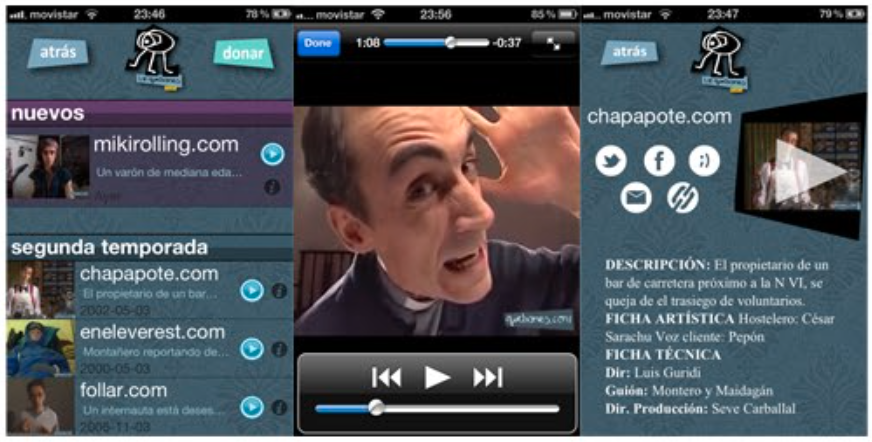
\includegraphics[width=\linewidth]{images/guebones.png}
				\end{minipage}

			\end{job}


			\begin{job}[6/2012 \\ - \\11/2012]

				\begin{minipage}{0.65\linewidth}
					\textbf{iOS Developer at deexMe}

					Development of a prototype (with almost all functionality) of the iPhone app for the social network Deexme. I developed quite complex UI layouts and integrated it with several APIs.
				\end{minipage}\hspace*{0.05\linewidth}\begin{minipage}{0.3\linewidth}
					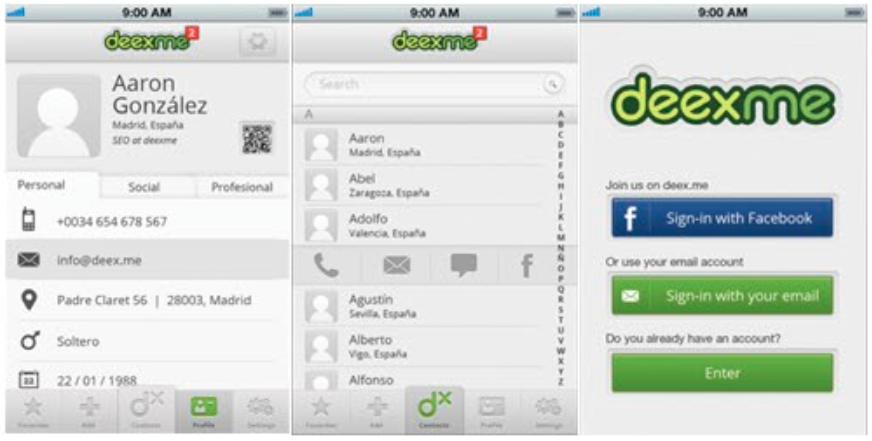
\includegraphics[width=\linewidth]{images/deexme.png}
				\end{minipage}
				
			\end{job}

			\begin{job}[5/2013 \\ - \\9/2013]

				\begin{minipage}{0.65\linewidth}
					\textbf{Research intern at IMDEA Software Madrid}

					I helped program a static assembly analyzer that would derive leackage upper bounds for different cache-related sidechannel attacks. Also run some experiments with popular encription algorithms.
				\end{minipage}\hspace*{0.05\linewidth}\begin{minipage}{0.3\linewidth}
					
\includegraphics[width=\linewidth]{images/imdea.png}
				\end{minipage}

			\end{job}

			\begin{job}[2/2014 \\ - \\5/2014]

				\begin{minipage}{0.65\linewidth}
					\textbf{Remote freelancer with oDesk}

					I signed up in oDesk and worked with 3 clients. The one I spent most time with was \textbf{Mediafire} helping them add features to their internal management tool. I worked primarily with jQuery and php. The other two projects were a simple guided custom search box and a prototype for a health-tracking website which I did with angularjs and RoR.

				\end{minipage}\hspace*{0.05\linewidth}\begin{minipage}{0.3\linewidth}
					
\includegraphics[width=\linewidth]{images/odesk.png}
				\end{minipage}
			\end{job}

			\begin{job}[6/2014 \\ - \\1/2015]
			
				\begin{minipage}{\linewidth}
					\textbf{Remote frontend web developer at Qandell}

					I developed a complete frontend for the Qandell API with angularjs. It is a quite complex app, with lots of specific interfaces for data input. I had to include support for compressing images and parsing excel files on the browser. This project led me to a couple of angular libraries. One already released on bower. The website has not been released yet.

				\end{minipage}
			\end{job}

			\begin{job}[9/2014 \\ - \\12/2015]
			
				\begin{minipage}{0.65\linewidth}
					\textbf{Intern in the department of innovative education at UAM}

					I colaborated in the creation of the MOOCs published by UAMx in the platform edX. My responsibilities included the creation of interactive web tools to enhance the learning experience and to make things clearer for students. I also had to recreate some existing flash elements using HTML5. I was also taking care of material usage rights.

				\end{minipage}\hspace*{0.05\linewidth}\begin{minipage}{0.3\linewidth}
					
\includegraphics[width=\linewidth]{images/uam.jpg}
				\end{minipage}
			\end{job}

		\end{timeline}


\end{document}
